\section{Proving}
\label{tut_proving}
\index{proving}

\tick{\textbf{Goals:} The goal of this section is to get familiar with the Proving Perspective and to carry out a simple proof by hand.  It also introduces more sophisticated data structures than the ones we introduced so far.}

\subsection{The Celebrity Problem}
\label{tut_celebrity_problem}

In this section, we will work with the model of the so-called celebrity problem.

\warning{We are using a new model instead of the traffic light because it provides us with some proofs where manual interaction is necessary.}

In the setting for this problem, we have a ``knows'' relation between persons.
This relation is defined so that

\begin{itemize}
	\item no one knows himself,
	\item the celebrity knows nobody,
	\item everybody knows the celebrity.
\end{itemize}    

The problem's goal is to find the celebrity. We want to model an algorithm that fulfills this task.

\subsection{Importing a project}
\label{tut_import_project}
\index{import project}

Rather than creating the model step by step, we have provided the model as an archive file.

\warning{Make sure that you have no existing Project named ``Celebrity'', before importing the project. If you have, then rename it by right clicking the project and selecting \textsf{Rename...}}

Import the archive file \file{Celebrity.zip}{Celebrity.zip} to you Event-B Explorer. To do this, select \textsf{File $\rangle $ Import $\rangle $ General $\rangle $ Existing Projects into Workspace}. Then select the option to import an existing archive file. Use the browse function to find your archive file and import it. After you have selected the appropriate archive file, click on \textsf{Finish}.

It will take a few seconds for Rodin to extract and load all the files. Once this is done, a few problems will be displayed in the Rodin Problems view (compare with Figure \ref{fig_tut_08_rodin_problemview}).

\begin{figure}[!ht]
\begin{center}
	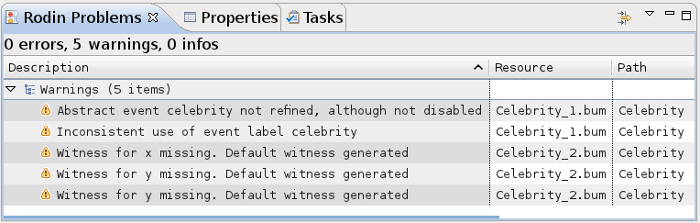
\includegraphics{img/tutorial/tut_08_rodin_problems.png}
	\caption{Warnings in the Rodin Problems View}
	\label{fig_tut_08_rodin_problemview}
\end{center}
\end{figure}

We will describe how the model is organized below in Section \ref{the_celebrity_algorithm}.  But before we do so, we will fix the existing problems.

\subsection{Fixing Problems}
\label{tut_celebrity_fixing problems}
\index{warnings}

Before proceeding, we will fix the problems shown in Figure \ref{fig_tut_08_rodin_problemview}. Let's take a look at the warning stating that the event label ``celebrity'' is misused (``Inconsistent use of event label celebrity''). Double-click on this warning to open the \texttt{Celebrity\_1} machine. The line with the error is already underlined in yellow\footnote{This is the behaviour of the default editor.  Other editors may exhibit a different behaviour}. This error is produced by the event called \textsf{celebrity}.

The problem is that the event is not declared as a refinement. To solve the problem, add an \textsf{Event-B Refines Event Relationship} child which will add a new entry in the \textsf{REFINES} section.  To do so, right-click in the empty space to the left of the word \textsf{celebrity} or place your cursor directly to the left of the small green arrow (\icon{rodin/structured_arrow.png}) and right-click. Now select \textsf{Add Child $\rangle$ Event-B Refines Event Relationship}.

\warning{Make sure that the cursor is on the correct line before right-clicking.  Otherwise, you will get the wrong context menu.  Also, make sure that you are not in ``text edit'' mode (e.g. clicking on a word like ``celebrity'' that you can edit will bring you into ``text edit'' mode).  This will give you the wrong context menu as well. See the faq for more info (\ref{faq_new_editor_new_element}).}

 This declares that the event is a refinement of an event with the same name in the abstract machine (\ref{abstract_machine}). This is the case here, so we can now save the project and the warning should disappear.

%Do we need an additional explanation for witnesses, since this is already done in tutorial 07!?
%In any abstract event that uses parameters, if the concrete event has no parameter with the same name, the tool needs a witness so that it notices what value the parameter should take. Witnesses are also needed for variables that have a non-deterministic (\ref{non_deterministic}) assignment in an abstract event and do not appear in the concrete model.

The three remaining warnings state that witnesses (\ref{witness}) are missing. Double click on the warning to open the concrete model (here \texttt{Celebrity\_2}). Then add an \textsf{Event-B Witness} child to the event called \textsf{celebrity}.

A default witness \textsf{wit1} has been created, with a default value \textsf{$\btrue$} (e.g. the predicate ``true'') which we need to change. The name of a witness has to be the same as the parameter of the corresponding abstract event that it is refining. Here the name of the witness will have to be \textsf{x} so that it can be a witness for the parameter \textsf{x} of the corresponding abstract event in the machine \texttt{Celebrity\_1}. The abstract event has the assignment \textsf{$r \bcmeq x$}, while the concrete one has the assignment \textsf{$r \bcmeq b$}. So the content of the witness should \textsf{b = x}. The event should now look as follows: 

\begin{description}
	\EVT {celebrity}
	\REF {celebrity}
		\begin{description}
		\WhenGrd
			\begin{description}
			\nItemX{ grd1 }{ R = \emptyset  }
			\end{description}
		\Witnesses
			\begin{description}
			\nItem{ x }{ b=x }
			\end{description}
		\ThenAct
			\begin{description}
			\nItemX{ act1 }{ r :=  b }
			\end{description}
		\EndAct
		\end{description}
\end{description}

Edit the content and save the file. One warning will disappear, and only two will remain.

\info{
Try completing the other two witnesses on your own. A hint: Both witnesses are simple equalities, and both can be found by comparing the third guard of the abstract event with the second guard of the concrete one. Remember to give the witness the name of the variable it stands for. If you completed this step correctly, there should be no warning, info or error left in the Rodin Problems view (\ref{rodin_problems_view}).
}

The following section (\ref{tut_final_second_refinement}) shows the corrected \texttt{Celebrity\_2} machine.

\subsection{The Final Second Refinement}
\label{tut_final_second_refinement}

\pencil{
\begin{description}
\MACHINE{Celebrity\_2}
\REFINES{Celebrity\_1}
\SEES{Celebrity\_c0}
\VARIABLES
	\begin{description}
		\Item{ r }
		\Item{ R }
		\Item{ b }
	\end{description}
\INVARIANTS
	\begin{description}
		\nItemX{ inv1 }{ R \subseteq  P }
		\nItemX{ inv2 }{ b \in  P }
		\nItemX{ inv3 }{ b \notin  R }
		\nItemX{ inv4 }{ Q = R \bunion  \{ b\}  }
	\end{description}
\EVENTS
	\INITIALISATION
		\begin{description}
		\BeginAct
			\begin{description}
			\nItemX{ act1 }{ r :\in  P }
			\nItemX{ act2 }{ b, R :|  b' \in  P \land  R' = P \setminus  \{ b'\}  }
			\end{description}
		\EndAct
		\end{description}
	\EVT {celebrity}
	\REF {celebrity}
		\begin{description}
		\WhenGrd
			\begin{description}
			\nItemX{ grd1 }{ R = \emptyset  }
			\end{description}
		\Witnesses
			\begin{description}
			\nItem{ x }{ b=x }
			\end{description}
		\ThenAct
			\begin{description}
			\nItemX{ act1 }{ r :=  b }
			\end{description}
		\EndAct
		\end{description}
	\EVT {remove\_1}
	\REF {remove\_1}
		\begin{description}
		\AnyPrm
			\begin{description}
			\ItemX{ x }
			\end{description}
		\WhereGrd
			\begin{description}
			\nItemX{ grd1 }{ x \in  R }
			\nItemX{ grd2 }{ x \mapsto  b \in  k }
			\end{description}
		\Witnesses
			\begin{description}
			\nItem{ y }{ b=y }
			\end{description}
		\ThenAct
			\begin{description}
			\nItemX{ act1 }{ R :=  R \setminus  \{ x\}  }
			\end{description}
		\EndAct
		\end{description}
	\EVT {remove\_2}
	\REF {remove\_2}
		\begin{description}
		\AnyPrm
			\begin{description}
			\ItemX{ x }
			\end{description}
		\WhereGrd
			\begin{description}
			\nItemX{ grd1 }{ x \in  R }
			\nItemX{ grd2 }{ x \mapsto  b \notin  k }
			\end{description}
		\Witnesses
			\begin{description}
			\nItem{ y }{ b=y }
			\end{description}
		\ThenAct
			\begin{description}
			\nItemX{ act2 }{ b :=  x }
			\nItemX{ act1 }{ R :=  R \setminus  \{ x\}  }
			\end{description}
		\EndAct
		\end{description}
\END
\end{description}
}
\subsection{The Celebrity algorithm}
\label{the_celebrity_algorithm}

We will now take a brief tour through the model to see how the problem and algorithm are specified.
The celebrity problem itself is described in the context \texttt{Celebrity\_c0}. There are
  three constants. $P$ is the set of persons, each represented by a number, $c$ is the celebrity
  we are looking for and $k$ is the ``knows'' relation between the persons.
The axioms encode the properties about the ``knows'' relation that we stated above.

\pencil{
\begin{description}
\CONTEXT{Celebrity\_c0}
\CONSTANTS
	\begin{description}
		\Item{ k }
		\Item{ c }
		\Item{ P }
	\end{description}
\AXIOMS
	\begin{description}
		\nItemX{ axm1 }{ P \subseteq  \nat }
		\nItemX{ axm2 }{ c \in  P }
		\nItemX{ axm3 }{ k \in  (P \setminus  \{ c\} ) \rel  P }
		\nItemX{ axm4 }{ k^{-1}  [\{ c\} ] = P \setminus  \{ c\}  }
		\nItemX{ axm5 }{ k \binter  id = \emptyset  }
	\end{description}
\END
\end{description}
}

In the most abstract machine \texttt{Celebrity\_0} we specify what the algorithm should do.
The variable $r$ can be any person initially and the event \texttt{celebrity} 
  finds the celebrity in one step. 
After the event \texttt{celebrity} has occurred, $r$ contains the result of the algorithm.
You might then wonder why there is a problem if you can just pick the celebrity and assign it to the result. This is because we defined our problem in such a way so that we are certain a celebrity $c$ exists and the algorithm simply returns it.
Later in the refinement, we will model how to find the celebrity without using $c$.
Because of the refinement relation, we know that the algorithm works correctly.

\pencil{
\begin{description}
\MACHINE{Celebrity\_0}
\SEES{Celebrity\_c0}
\VARIABLES
	\begin{description}
		\Item{ r }
	\end{description}
\INVARIANTS
	\begin{description}
		\nItemX{ inv1 }{ r \in  P }
	\end{description}
\EVENTS
	\INITIALISATION
		\begin{description}
		\BeginAct
			\begin{description}
			\nItemX{ act1 }{ r :\in  P }
			\end{description}
		\EndAct
		\end{description}
	\EVT {celebrity}
		\begin{description}
		\BeginAct
			\begin{description}
			\nItemX{ act1 }{ r :=  c }
			\end{description}
		\EndAct
		\end{description}
\END
\end{description}
}

So let's have a look at the first refinement \texttt{Celebrity\_1}. 
A variable $Q$ is introduced which contains a subset of the persons, the potential celebrities.
We start with $Q$ being all persons.
Two new events,  \texttt{remove\_1} and \texttt{remove\_2}, are added to remove people
  from $Q$ who cannot be the celebrity.
\texttt{remove\_1} removes a person that knows somebody while \texttt{remove\_2}
  removes a person that is not known by any other person.
An invariants states that the celebrity is always in $Q$.
When there is just one person left in the set, we know that this is the celebrity.

The second refinement, \texttt{Celebrity\_2}, then splits the
  potential celebrities $Q$ into one arbitrary person -- the candidate $b$ --
  and the ``rest'' $R$.
\texttt{remove\_1} then removes a person $x$ from $R$ if $b$ knows $x$.
\texttt{remove\_2} checks if there is a person $x$ in $R$ that does not know the candidate.
If found, $x$ is the new candidate $b$ and is removed from the rest $R$.
If $R$ is empty, we know that the candidate is the celebrity. (We do not show the machine here because it simply takes up too much space --- please consult the project that you imported earlier to inspect the model.)

The third refinement then makes some more assumptions about the given problem.
The context \texttt{Celebrity\_c1} extends \texttt{Celebrity\_c0} and states that
  there are $n+1$ persons with the numbers $0\upto n$.

\pencil{
\begin{description}
\CONTEXT{Celebrity\_c1}
\EXTENDS{Celebrity\_c0}
\CONSTANTS
	\begin{description}
		\Item{ n }
	\end{description}
\AXIOMS
	\begin{description}
		\nItemX{ axm1 }{ n \in  \nat }
		\nItemX{ axm2 }{ n >  0 }
		\nItemX{ axm3 }{ P = 0\upto n }
	\end{description}
\END
\end{description}
}

Instead of having an abstract data structure like a set, the third refinement just introduces
  an index variable $a$ that points to the first person of $R$, which is the group of people who have not yet been checked.
Instead of taking an arbitrary element from $R$ as in the second refinement, the remove
  events just takes the first element $a$. $a$ is then removed from $R$ by increasing
  it by one.
When $a$ is larger then $n$, $R$ is empty and $b$ contains the result.

This last refinement works only on the following three integer variables: 
The index $a$, the candidate $b$ and the result $r$.
Each event is deterministic and in every step only one event is enabled.
The events together can be interpreted as an implementation of the algorithm:
\newline

\begin{tabular}{ll}
  $r \bcmeq 0$ & // initialisation \texttt{act1} \\
  $a \bcmeq 1$ & // initialisation \texttt{act2} \\
  $b \bcmeq 0$ & // initialisation \texttt{act3} \\
  \textbf{while} $a\leq n$ \textbf{do} & // guard in \texttt{remove\_1} and \texttt{remove\_2}\\
  \quad \textbf{if} $a\mapsto b\in k$ \textbf{then} & // guard in \texttt{remove\_1} and negated in \texttt{remove\_2}\\
  \qquad $a \bcmeq a+1$ & // action in \texttt{remove\_1} \\
  \quad \textbf{else} & // $a\mapsto b\not\in k$\\
  \qquad $b \bcmeq a$ & // action \texttt{act1} in \texttt{remove\_2} \\
  \qquad $a \bcmeq a+1$ & // action \texttt{act2} in \texttt{remove\_2} \\
  \quad \textbf{end if} \\
  \textbf{end while} \\
  $r \bcmeq b$ & // action in \texttt{celebrity}
\end{tabular}

\subsection{The First Proof}
\label{tut_first_proof}

In this section, we will carry out proofs for the model of the Celebrity Problem. To do this, click on the box in the upper right hand corner that has a little plus sign and switch to the Proving Perspective. You can switch between perspectives using the shortcut bar as shown in Figure \ref{fig_tut_08_switch_perspective}. 

\begin{figure}[!ht]
\begin{center}
	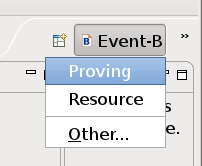
\includegraphics{img/tutorial/tut_08_switch_perspective.png}
	\caption{Switch Perspective}
	\label{fig_tut_08_switch_perspective}
\end{center}
\end{figure}

\warning{If the Proving Perspective is not available in the menu, select \textsf{Other... $\rangle$ Proving}. This will open a new window which shows all available perspectives.}

We should now see the window in Figure \ref{fig_tut_08_proving_perspective}. 

\begin{figure}[!ht]
\begin{center}
	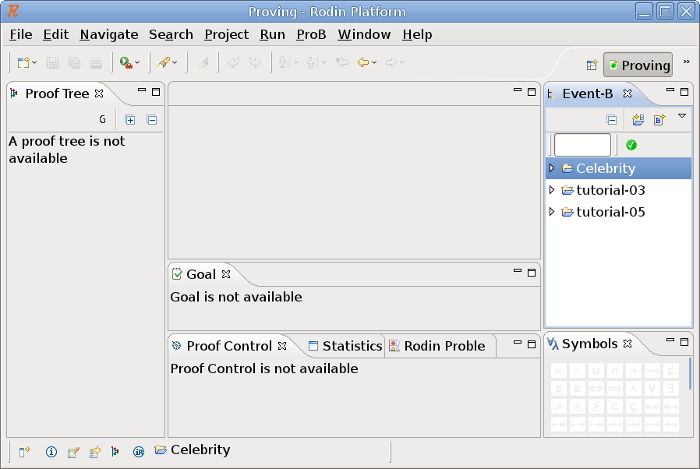
\includegraphics{img/tutorial/tut_08_proving_perspective.png}
	\caption{Rodin Proving Perspective}
	\label{fig_tut_08_proving_perspective}
\end{center}
\end{figure}

The \texttt{Proving Perspective} contains three new important views:

\begin{description}
	\item[Proof Tree View (\ref{proof_tree_view})] Here we see a tree of the proof that we have done so far and the current position in it. By clicking in the tree, we can navigate within the proof. We have not yet started the proof, so there is nothing to see yet.
	\item[Proof Control View (\ref{proof_control_view})] This is where we perform interactive proofs.
	\item[Goal View (\ref{goal_view})] This window shows what needs to be proved at the current position inside the proof tree.
\end{description}

Expand the \texttt{Celebrity\_1} machine in the \textsf{Event-B Explorer}. Then expand the \textsf{Proof Obligations} section. We can see that the auto prover (\ref{auto_prover}) did quite a good job. Only three proofs have not been completed\footnote{Interestingly enough, this number can vary: Provers can be configured in the preferences and changes there can have an impact on the ability to automatically discharge proofs.  In addition, all provers have timeouts.  On a slow machine, some proof obligations may not be discharged whereas on a faster machine with the same timeout they would be discharged.}  (a completed proof is indicated by a green check \icon{rodin/discharged.png}). 

%Except for the last one of them, all of them could be proved with a different external prover, but in order to learn a few new techniques, we will prove them with the so called ``p0 prover'' (\ref{p0_prover}). The p0 prover uses all selected hypotheses (the ones in Selected Hypotheses View).

\info{Each proof has a label, e.g. \textsf{remove\_1/inv2/INV}.  Proof labels are explained in Section~\ref{generated_proof_obligations}.}
Let's start with the proof \textsf{remove\_1/inv2/INV} of \texttt{Celebrity\_1}.
To do this, double click on the proof obligation \textsf{remove\_1/inv2/INV}.
We should now see the window as shown in Figure \ref{fig_tut_08_proof_obligation}.

%\begin{figure}[!ht]
%\begin{center}
%	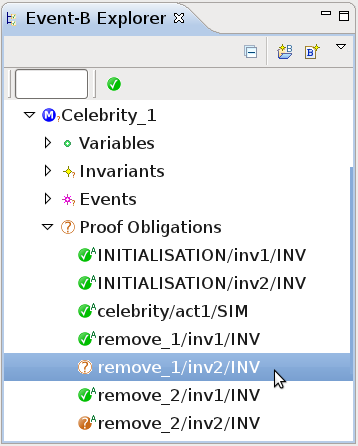
\includegraphics{img/tutorial/tut_08_proof1.png}
%	\caption{Rodin Proving Perspective}
%	\label{fig_tut_08_proving_perspective}
%\end{center}
%\end{figure}

\begin{figure}[!ht]
\begin{center}
	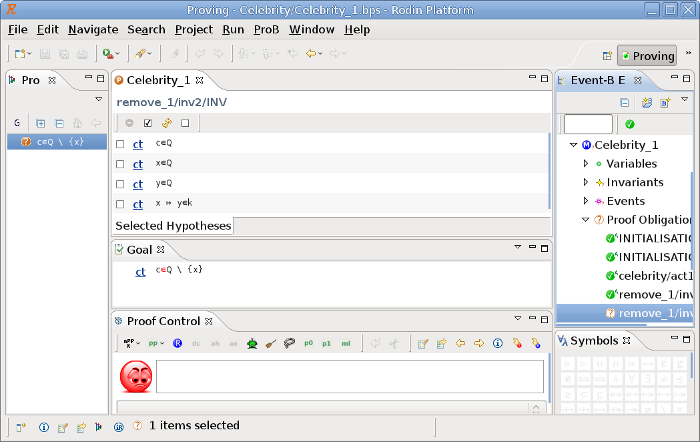
\includegraphics{img/tutorial/tut_08_proof2.png}
	\caption{Proof Obligation}
	\label{fig_tut_08_proof_obligation}
\end{center}
\end{figure}

\info{Make sure that you understand the different buttons in the \textsf{Proof Control View} (\ref{proof_control_view}).}

Here we need to prove that the event \texttt{remove\_1} preserves the invariant \texttt{inv2},
  $c\in Q$.
The event's action assigns the new value $Q\setminus \{x\} $to $Q$.
Because we know that invariant $c\in Q$ was valid before the assignment, 
 it is sufficient to prove that we do not remove $c$ from $Q$, i.e. \textsf{$x \neq c$}. Type this into the \textsf{Proof Control View} (\ref{proof_control_view}) and press the \textsf{\icon{rodin/ah_prover.png} button}. 

\info{In order to undo a step, click on a node in the \texttt{Proof Tree View} and click on the \icon{rodin/pn_prover.png} button in the \texttt{Proof Control View} or open the context menu of a node and select \texttt{Prune}.}

Take a look at the Proof Tree View. The root node should now be labeled with \texttt{ah ($x\neq c$)},
  which is the hypothesis that we just added.
This node has three children: The first proves that $x\neq c$ is well-defined, which is $\btrue$ and has already been trivially proven.\marginpar{(mj) ... and how do we know that this used to be the WD proof obligation?  This information seems to be lost.}
The second is the proof of the hypotheses $\lnot x=c$.
The third is the proof of the original goal where the new hypotheses can be used.

The new goal is $\lnot x = c$. Now, try selecting the right hypotheses by yourself in order to complete the proof (Hint: What axiom states that the celebrity does not know anybody?). To do this, click on the \icon{rodin/sh_prover.png} button in the \textsf{Proof Control View}. On the left side we should see now the \textsf{Search Hypotheses} view (see Figure \ref{fig_tut_08_search_hypothesis}). If you cannot find the right hypotheses, you may also just select all hypotheses. To add the selected hypothesis to the \textsf{Selected Hypotheses View} just click on the \icon{rodin/add.png} button. 

\info{There is usually no harm in selecting all hypothesis, but this approach is not optimal.  By providing only necessary hypotheses and no more, we drastically increase the chance that the prover will find the solution before timing out.  On large models it is next to impossible to prove everything without hand-picking the hypotheses.}

\begin{figure}[!ht]
\begin{center}
	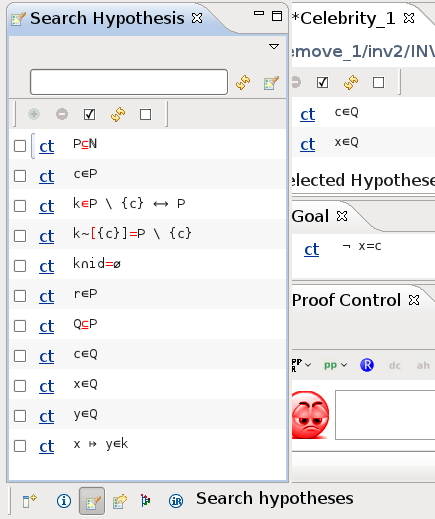
\includegraphics{img/tutorial/tut_08_search_hypothesis.png}
	\caption{Search Hypothesis View}
	\label{fig_tut_08_search_hypothesis}
\end{center}
\end{figure}

The correct hypothesis for this proof was $k \in  (P \setminus  \{ c\} ) \rel  P$ (axiom 3 from the first context). If you were unable to figure this out, add this hypothesis to the selected hypothesis window now. Now click on the \icon{rodin/p0.png} button to prove the goal $\lnot x = c$ with the \textsf{Predicate prover on selected hypothesis}. The goal should be discharged and in the Proof Tree you should see that the first two children of the root node are proven. The \textsf{Proof Control View} should now show the original goal $c \in Q \setminus {x}$ and $x\neq c$ is now one of our hypotheses.\footnote{The prover has rewritten this as $ \lnot x = c$} Click a second time on the \icon{rodin/p0.png} button in order to finalize the proof. The smiley in the \textsf{Proof Control View} should now become green indicating that all sequents of the proof tree are discharged as shown in Figure \ref{fig_tut_08_proof_final}.

\begin{figure}[!ht]
\begin{center}
	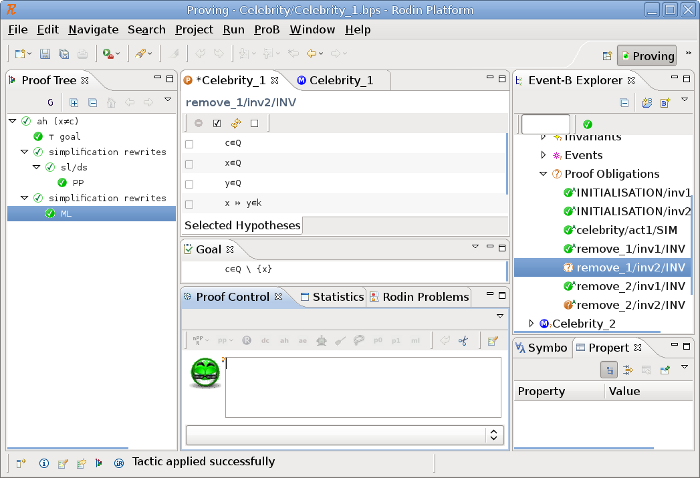
\includegraphics{img/tutorial/tut_08_proof_final.png}
	\caption{The green smiley indicates that all sequents of the proof tree are discharged}
	\label{fig_tut_08_proof_final}
\end{center}
\end{figure}

After saving the proof, the proof obligation \textsf{remove\_1/inv2/INV} in the \textsf{Event-B Explorer} should now have a \icon{rodin/discharged.png} next to it.

\info{Those proof obligations that were automatically discharged are marked with a tiny ``A'' next to the \icon{rodin/discharged.png}.  As the one we just discharged was proven manually, this is now the first discharged PO without an ``A''.}

\info{There are alternative ways to prove the proof obligation. For instance, we can use the \icon{rodin/lasoo_prover.png} button to load all hidden hypotheses that contain identifiers in common with the goal into the \textsf{Selected Hypotheses View}, and we can also use it with the selected hypotheses.}

In order to move to the next undischarged proof obligation, you may also use the \textsf{Next Undischarged PO button} (\icon{rodin/next_prover.png}) of the \textsf{Proof Control View} (\ref{proof_control_view}). The next proof can be solved the same way as the last one.

\info{As an exercise, try to prove \texttt{Celebrity\_2}. A small hint: To do this, we have to fill in an existential quantifier. We need to instantiate \textsf{b'} correctly. The auto prover should have proved that $b' \in P$, so look for a variable that is already in P and add this value to the \textsf{Selected Hypotheses View}. To instansiate \textsf{b'}, type the name of the variable you have chosen into the yellow box that is shown in the \textsf{Goal View} (\ref{goal_view}) and then click on the red existential quantifier. Now all open branches of the proof tree can be proved with the \icon{rodin/p0.png} prover. After this, we have completed all the proofs, and the model is ready for use. } 

\subsection{Proving --- an Art or a Science?}
\label{tut_proving_an_art_or_a_science}

Proving can be quite frustrating for both beginners and advanced users.  Beginners sometimes get the impression that proving is just ``clicking around'' that sometimes works and sometimes does not.  When it does work, it's not really clear why. The proof tree is also difficult to read even for experienced users.  We provided some additional guidance on provers in the reference chapter (\ref{use_provers_effectively}) that may be of help, but keep in mind that proving is a skill that can only be learned by practice. Here we are trying to help you learn how you can use Rodin to solve proofs, but actually teaching you how to prove something is not really in the scope of this document.


%%% Local Variables: 
%%% mode: latex
%%% TeX-master: "rodin-doc"
%%% End: 
